\chapter{Chemical shifts in a probabilistic framework}

This section introduces the formalism for Monte Carlo simulations which includes both physical energy terms as well as a probabilistic energy terms based on experimentally observed chemical shifts.
These equations presented are not new, but have not been published in the form in which they are presented here.
The intention is to present the equations in the form in which they are implemented in PHAISTOS,  so that they can easily be re-implemented in other programs by others.

\section{Defining an energy function from Bayes' theorem}
A simplistic approach to this problem is to is to define a hybrid energy by defining a penalty function that describes the agreement between experimental data and data calculated from a proposed protein structure with a physical energy (such as from a molecular mechanics force field).
A structure is then determined by minimizing
\begin{equation}
E_{\mathrm{hybrid}}= w_{\mathrm{data}}\ E_{\mathrm{data}}+E_{\mathrm{physical}}.
\end{equation}
This approach, however, does not uniquely define neither shape nor weight of $E_{\mathrm{data}}$.
Chemical shifts have been combined with physical energies in a multitude of ways, e.g., weighted RMSD values or harmonic constraints.
Vendruscolo and co-workers implemented a "square-well soft harmonic potential", and corresponding molecular gradients and were able to run a chemical shift-biased MD simulation.
In all cases the parameters and weights of $E_{\mathrm{data}}$ had to be carefully tweaked by hand, and it is not clear how to choose optimal parameters.

The inferential structure determination (ISD) principles introduced by Rie-ping, Habeck and Nigles \cite{Rieping2005}defines a Bayesian formulation of Eq XX. In the following section the equations of an ISD approach are derived for combining the knowledge of experimental chemical shifts with a physical energy. First remember Bayes' theorem which relates a conditional probability ($A$ given $B$) with its inverse:
\begin{equation}
p\left(A | B \right) =\frac{p\left(B | A \right)p\left(A\right)}{p\left(B \right)} 
\end{equation}
Now consider a set of chemical shifts $\{\delta_i\}$, and the uncertainty to which these can be predicted $\{\sigma_i\}$ from a structure, $\mathbfit X$ (the experimental uncertainty is negligibly small compared to this). We have to make the basic assumption, that the error, given as $\Delta\delta_i = \left| \delta_i^{\mathrm{predicted}} - \delta_i^{\mathrm{experimental}}\right|$, approximately follows a Gaussian distribution with some standard deviation, but we need not hand-pick and assign any numeric value to the standard deviation.Furthermore, the Gaussian distribution is the least biasing distribution according to the principle of maximum entropy.


In this case, the most likely structure, $\mathbfit X$, and optimal choice of $\{\sigma_i\}$ is found by maximizing (via Bayes' theorem)
\begin{equation}
p\Big(\mathbfit X, \{\sigma_i\} \Big| \{\delta_i\} \Big) = \frac{p\Big( \{\delta_i\} \Big| \mathbfit X, \{\sigma_i\}\Big)p\Big(\mathbfit X, \{\sigma_i\} \Big)}{p\Big( \{\delta_i\}\Big)}.
\end{equation}\\
Here, \textit{marginal distribution} of $p\left( \{\delta_i\}\right)$ merely serves as a normalizing factor and the \textit{likelihood} of $p\left( \{\delta_i\} | \mathbfit X, \{\sigma_i\}\right)$, is obtained as the product of the individual, Gaussian probabilities over all $n$ single chemical shift measurements. Nuclei of the same atom-type, here denoted by index $j$, (e.g. C$^\alpha$, H$^\alpha$, etc.) are assumed to carry the same uncertainly denoted by $\sigma_j$:

\begin{eqnarray}
p\Big( \{\delta_i\} \Big| \mathbfit X, \{\sigma_i\}\Big) &\simeq& \prod_{i=0}^{n} p\left( \Delta\delta_i | \mathbfit X, \sigma_i \right)\\
& = & \prod_{j=0}^{m} \prod_{i_j=0}^{n_j} p\left( \Delta\delta_{i_j} | \mathbfit X, \sigma_j \right)\\
& = & \prod_{j=0}^{m} \prod_{i_j=0}^{n_j} \frac{1}{\sigma_j \sqrt{2\pi}} \exp{ \left( - \frac{\Delta\delta_{i_j}^2}{2\sigma_j^2} \right) }\\
& = & \prod_{j=0}^{m} \left( \frac{1}{\sigma_j \sqrt{2\pi}}\right)^{n_j} \exp{ \left( \sum_{i_j=0}^{n_j} - \frac{\Delta\delta_{i_j}^2}{2\sigma_j^2} \right) }\\
& = & \prod_{j=0}^{m} \left( \frac{1}{\sigma_j \sqrt{2\pi}}\right)^{n_j} \exp{ \left(  \frac{- \chi_j^2(\mathbfit X)}{2\sigma_j^2}\right) }
\end{eqnarray}\\
Furthermore, $p\left(\mathbfit X, \{\sigma_j\} \right)$ can be simplified as 

\begin{eqnarray}
p\Big(\mathbfit X, \{\sigma_j\} \Big) & \propto & p\Big(\{\sigma_j\} \Big| \mathbf X \Big) p\Big(\mathbf X\Big)\\
& = & p\Big(\{\sigma_j\} \Big) p\Big(\mathbfit X\Big),
\end{eqnarray}
where it is assumed that the errors in the chemical shift prediction model are independent of the particular protein structure and \textit{vice versa}. The \textit{prior} distribution of $p\left(\{\sigma_j\} \right)$ is accounted for by proposing updates from a log-normal distribution (see next subsection). $p(\mathbfit X)$ of the molecular protein structure is here simply the Boltzmann distribution, i.e. 
\begin{equation}
p(\mathbfit X) = \frac{1}{Z}\exp{\left(-\frac{E(\mathbfit X)}{k_\mathrm{B}T}\right)}
\end{equation}\\
where $E(\mathbfit X)$ is the (physical) potential energy of the protein structure, most often described by a molecular mechanics force field. $k_\mathrm{B}$ is the Boltzmann constant and $T$ is the temperature of interest. Luckily we need not calculate the partition function, $Z$, because the relative energy landscape is invariant under choice of normalization constant. Note that $p(\mathbfit X)$ also can be introduced via conformational sampling from a biased distribution, such as for example TorusDBN or BASILISK (mimicking the Ramachandran plot and side chain rotamer distributions, respectively). 
\\\\
Neglecting normalization constants, the total probability to be maximized is thus proportional to:
\begin{eqnarray}
&&p\Big( \mathbfit X, \{\sigma_i\} \Big| \{\delta_i\} \Big)  \propto  p\Big( \{\delta_i\} \Big| \mathbfit X, \{\sigma_i\}\Big) p\Big(\mathbfit X\Big) p\Big(\{\sigma_i\} \Big) \\
&&\propto   \prod_{j=0}^{m} \left(\frac{1}{\sigma_j \sqrt{2\pi}}\right)^{n_j} \exp{ \left(  - \frac{1}{2\sigma_j^2} \chi_j^2 \right) } \exp{\left(-\frac{E(\mathbfit X)}{k_\mathrm{B}T}\right)} p\Big(\{\sigma_j\} \Big) 
\end{eqnarray}

When $p(\{\sigma_j\})$ is introduced via biased sampling, the associated hybrid-energy to be evaluated is (again neglecting constant terms) 
\begin{eqnarray}
E_{\mathrm{hybrid}}\left(\mathbfit{X}\right) &=&- k_\mathrm{B}T \ln{} \Big(p\Big( \mathbfit X, \{\sigma_i\} \Big| \{\delta_i\} \Big)\Big) \\
&= & E(\mathbfit X) - k_\mathrm{B}T \sum_{j=0}^{n_j}n_j \ln{} \left(\frac{1}{\sigma_j \sqrt{2\pi}} \right) + \frac{\chi_j^2}{2\sigma_j^2}
\end{eqnarray}


\subsection{Sampling of nuisance parameters}
Since the nuisance parameters of the energy functions are unknown, they too must be sampled.



\subsubsection{Jeffreys' prior (general, one-parameter case)}
The prior distribution of the nuisance parameter is inherently unknown.
In such cases, it is necessary to use a prior distribution that will have only very little influence on the sampled value.
One such \textit{uninformative prior} could for instance be a flat distribution over the positive real line.
The concept of Jeffreys' priors are a generalization of flat priors. In the one parameter case the Jeffrey's prior is given as 
\begin{eqnarray}
    p(\theta) \propto \sqrt{\mathbf{I}(\theta)},
\end{eqnarray}
where $\mathbf{I}(\theta)$ is the \textit{Fisher information} defined (in the one parameter case) as
\begin{eqnarray}
    \mathbf{I}(\theta) = \left\langle \left( \frac{\partial}{\partial\theta} \ln p(x|\theta) \right)^2 \right\rangle.
\end{eqnarray}


\subsubsection{Jeffreys' prior (Gaussian and Cauchy distributions)}
Here we derive Jefferys' prior for the uncertainty of a Gaussian distribution, i.e.~a distribution on the form
\begin{eqnarray}
    p(x|\mu, \sigma) = \frac{1}{\sqrt{2\pi\sigma^2}} \exp \left( \frac{-(x-\mu)}{2\sigma^2} \right).
\end{eqnarray}
This immediately gives us the Jeffreys' prior:
\begin{eqnarray}
    p(\sigma)
    & \propto & \sqrt{\left\langle \left( \frac{\partial}{\partial\sigma}
        \ln p(x|\mu, \sigma) \right)^2 \right\rangle}\nonumber\\
    & = & \sqrt{\left\langle \left( \frac{\partial}{\partial\sigma}
        \ln \left[\frac{1}{\sqrt{2\pi\sigma^2}} \exp \left( \frac{-(x-\mu)}{2\sigma^2} \right) \right]
        \right)^2 \right\rangle}\nonumber\\
%    & = & \sqrt{\left\langle \left( \frac{\partial}{\partial\sigma} \frac{-(x-\mu)}{2\sigma^2} \right)^2 \right\rangle}\\
    & = & \sqrt{\left\langle \left(\frac{(x-\mu) - \sigma^2}{\sigma^3} \right)^2 \right\rangle}\nonumber\\
    & = & \sqrt{\int^{\infty}_{-\infty}  p(x|\mu, \sigma) \left(\frac{(x-\mu) - \sigma^2}{\sigma^3} \right)^2 dx}\nonumber\\
    & = &\sqrt{ \frac{2}{\sigma^2}} \ \propto \ \frac{1}{\sigma}
\end{eqnarray}
\\\\Similarly for the $\gamma$ parameter of the Cauchy distribution of the form
\begin{eqnarray}
    p(x|x_0, \gamma) = \frac{1}{\pi\gamma\left[ 1 + \left(\frac{x-x_0}{\gamma} \right)^2\right]},
\end{eqnarray}
we obtain the following Jeffreys' prior:
\begin{eqnarray}
p(\gamma)
& \propto & \sqrt{\left\langle \left( \frac{\partial}{\partial\gamma}
    \ln p(x|x_0, \gamma) \right)^2 \right\rangle}\nonumber\\
& = & \sqrt{\left\langle \left( \frac{\partial}{\partial\gamma}
\ln \left[\frac{1}{\pi\gamma\left[ 1 + \left(\frac{x-x_0}{\gamma} \right)^2\right]} \right] \right)^2 \right\rangle}\nonumber\\
& = & \sqrt{\left\langle \left( -\frac{\gamma^2 - (x-x_0)^2}{\gamma^3 +\gamma(x-x_0)^2} \right)^2 \right\rangle }\nonumber\\
& = & \sqrt{\int^{\infty}_{-\infty}  p(x|x_0, \gamma) \left(  -\frac{\gamma^2 - (x-x_0)^2}{\gamma^3 +\gamma(x-x_0)^2}\right)^2 dx }\nonumber\\
& = & \sqrt{\frac{1}{2\gamma^2}} \ \propto \ \frac{1}{\gamma}
\end{eqnarray}








\begin{figure}%
    \centering
    \subfloat[Gaussian distribution]{
        {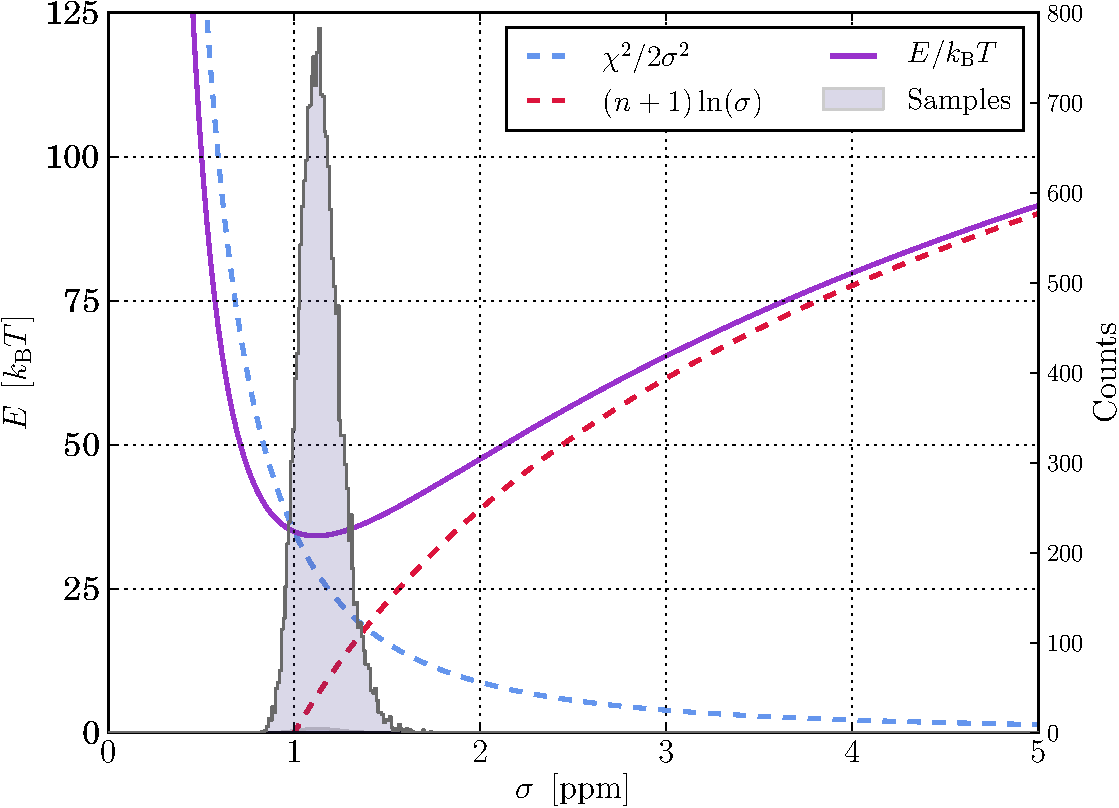
\includegraphics[width=0.45\textwidth]{figures/sigma_prior.pdf} }
    }
    \qquad
    \subfloat[Cauchy distribution]{
        {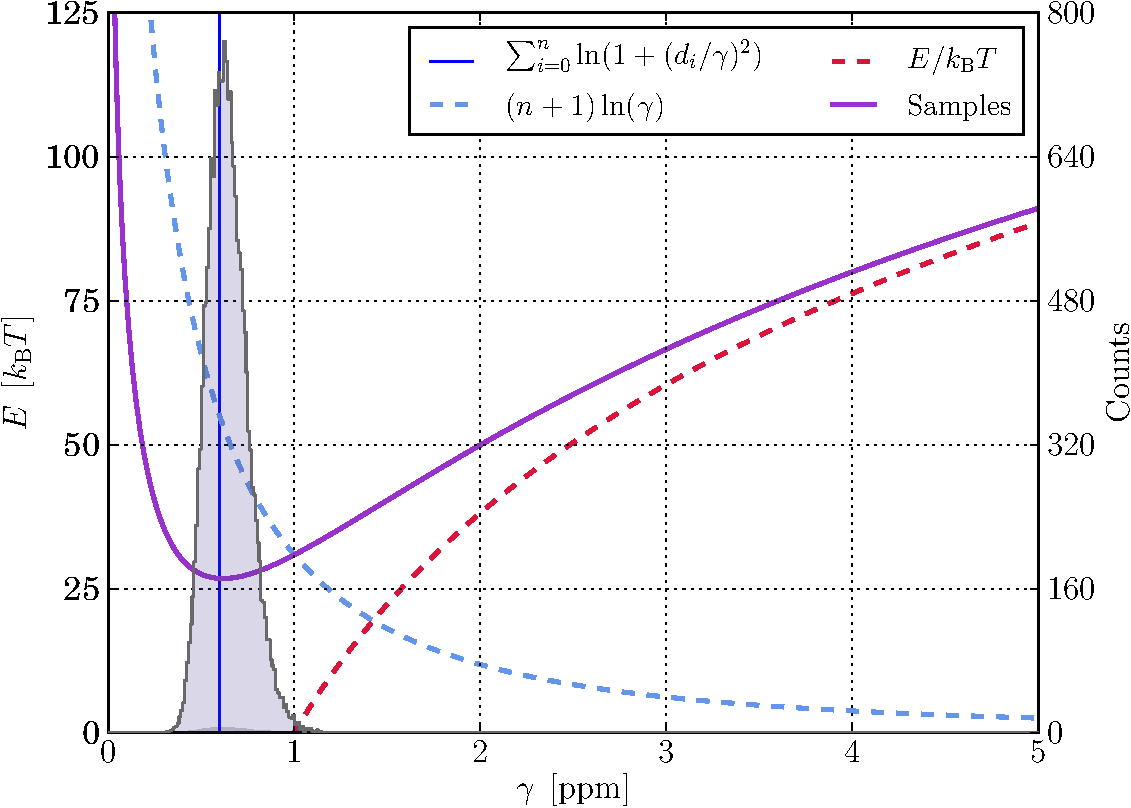
\includegraphics[width=0.45\textwidth]{figures/gamma_prior.pdf} }
    }
    \caption{Sampling of $\sigma$ and $\gamma$ for 2OED for Ca-chemical shifts. $n = 55$ and $\chi^2 = 69.7$.}
    \label{fig:example}%
\end{figure}
